% Organisers' ACM template (acmart, sigconf); template packages live in preamble.tex.
\documentclass[sigconf]{acmart}
% =============================================================================
% Template setup — participants normally do not edit this file.
% Author content belongs in main.tex; citations belong in main.bib.
% \documentclass lives in main.tex so Overleaf does not treat this file as root.
% =============================================================================

% --- Competition / non-ACM-submission friendly rights metadata ------------
\setcopyright{none}
\settopmatter{printacmref=false}
\acmConference[Kaggle Competition]{Filament Segmentation Challenge}{2026}{\href{https://www.kaggle.com/competitions/filament-segmentation-2026}{kaggle.com/competitions/filament-segmentation-2026}}
\acmBooktitle{Competition Report}
\acmDOI{}
\acmISBN{}

% --- Author guidance text --------------------------------------------------
% \guide{...} is gray italic while \guideStyletrue; omitted from the PDF if false.
% Flip the switch in main.tex after % =============================================================================
% Template setup — participants normally do not edit this file.
% Author content belongs in main.tex; citations belong in main.bib.
% \documentclass lives in main.tex so Overleaf does not treat this file as root.
% =============================================================================

% --- Competition / non-ACM-submission friendly rights metadata ------------
\setcopyright{none}
\settopmatter{printacmref=false}
\acmConference[Kaggle Competition]{Filament Segmentation Challenge}{2026}{\href{https://www.kaggle.com/competitions/filament-segmentation-2026}{kaggle.com/competitions/filament-segmentation-2026}}
\acmBooktitle{Competition Report}
\acmDOI{}
\acmISBN{}

% --- Author guidance text --------------------------------------------------
% \guide{...} is gray italic while \guideStyletrue; omitted from the PDF if false.
% Flip the switch in main.tex after % =============================================================================
% Template setup — participants normally do not edit this file.
% Author content belongs in main.tex; citations belong in main.bib.
% \documentclass lives in main.tex so Overleaf does not treat this file as root.
% =============================================================================

% --- Competition / non-ACM-submission friendly rights metadata ------------
\setcopyright{none}
\settopmatter{printacmref=false}
\acmConference[Kaggle Competition]{Filament Segmentation Challenge}{2026}{\href{https://www.kaggle.com/competitions/filament-segmentation-2026}{kaggle.com/competitions/filament-segmentation-2026}}
\acmBooktitle{Competition Report}
\acmDOI{}
\acmISBN{}

% --- Author guidance text --------------------------------------------------
% \guide{...} is gray italic while \guideStyletrue; omitted from the PDF if false.
% Flip the switch in main.tex after \input{preamble}.
%
% Do not use \guide{...} for \email{...}.
\usepackage{xcolor}
\newif\ifguideStyle
\guideStyletrue
\newcommand{\guide}[1]{%
  \ifguideStyle
    {\color{gray!65}\itshape #1}%
  \fi
}

% --- Math ------------------------------------------------------------------
% Do NOT load amssymb (or amsfonts): acmart already loads newtxmath, which
% defines the same symbols (e.g. \Bbbk) and causes a conflict on Overleaf.
% amsmath is already provided by acmart; mathtools extends it.
\usepackage{mathtools}

% --- Figures ---------------------------------------------------------------
% graphicx is already loaded by acmart
\usepackage{subcaption}

% --- Tables ----------------------------------------------------------------
% booktabs is already loaded by acmart
\usepackage{tabularx}
\usepackage{multirow}

% --- Bibliography style is set in main.tex (ACM-Reference-Format) ---------
.
%
% Do not use \guide{...} for \email{...}.
\usepackage{xcolor}
\newif\ifguideStyle
\guideStyletrue
\newcommand{\guide}[1]{%
  \ifguideStyle
    {\color{gray!65}\itshape #1}%
  \fi
}

% --- Math ------------------------------------------------------------------
% Do NOT load amssymb (or amsfonts): acmart already loads newtxmath, which
% defines the same symbols (e.g. \Bbbk) and causes a conflict on Overleaf.
% amsmath is already provided by acmart; mathtools extends it.
\usepackage{mathtools}

% --- Figures ---------------------------------------------------------------
% graphicx is already loaded by acmart
\usepackage{subcaption}

% --- Tables ----------------------------------------------------------------
% booktabs is already loaded by acmart
\usepackage{tabularx}
\usepackage{multirow}

% --- Bibliography style is set in main.tex (ACM-Reference-Format) ---------
.
%
% Do not use \guide{...} for \email{...}.
\usepackage{xcolor}
\newif\ifguideStyle
\guideStyletrue
\newcommand{\guide}[1]{%
  \ifguideStyle
    {\color{gray!65}\itshape #1}%
  \fi
}

% --- Math ------------------------------------------------------------------
% Do NOT load amssymb (or amsfonts): acmart already loads newtxmath, which
% defines the same symbols (e.g. \Bbbk) and causes a conflict on Overleaf.
% amsmath is already provided by acmart; mathtools extends it.
\usepackage{mathtools}

% --- Figures ---------------------------------------------------------------
% graphicx is already loaded by acmart
\usepackage{subcaption}

% --- Tables ----------------------------------------------------------------
% booktabs is already loaded by acmart
\usepackage{tabularx}
\usepackage{multirow}

% --- Bibliography style is set in main.tex (ACM-Reference-Format) ---------


\guideStylefalse

\begin{document}

\title[Real-Time Native-Resolution Filament Segmentation]{One Forward Pass at Native Resolution: Real-Time Solar Filament Segmentation with D-FINE-seg}
\subtitle{A Solution to the Solar Filament Segmentation Challenge 2026} % DO NOT CHANGE

\author{Argo Saakyan}
\affiliation{%
\institution{Agnify}
\city{Valencia}
\country{Spain}
}
\email{argo.cve@gmail.com}

\begin{abstract}
We segment solar filaments in full-disk GONG H$\alpha$ observations with a single small real-time network: a D-FINE-seg-S semantic segmentation model (8M parameters) applied once to the native $2048{\times}2048$ frame. Filament instances are the connected components of its probability map, and each is kept only if its mean probability is high, because Panoptic Quality (PQ) counts an unmatched prediction in its denominator and gains nothing from it. Scored against every annotator separately, the pipeline reaches PQ 0.429 on 144 held-out observations, against 0.334 for annotators scored against each other on the same observations, It agrees with the annotators better than they agree with each other on PQ, SQ, RQ and both Dice measures, with fragmentation and merging rates close to theirs. The public leaderboard score is 0.38. End to end, from JPEG to final masks, it takes 76\,ms per image on a consumer GPU with plain PyTorch and 1.5\,GB of allocated GPU memory. Input resolution was by far the largest gain (+0.057 PQ); larger models, instance segmentation, tiling, fusion, label variants, input preprocessing and test-time augmentation improved validation PQ by at most 0.005, at up to 20$\times$ the network time.
\end{abstract}

\maketitle

\section{Introduction}
This report describes our submitted solution to the Solar Filament Segmentation Challenge~2026 \cite{filament-segmentation-2026}, organised by the Earth-Space AI Research (ESAIR) Lab as part of the IEEE BigData~2026 Cup \cite{ieeebigdata2026cup}. The challenge uses the MAGFiLO dataset \cite{ahmadzadeh2024dataset} of GONG \cite{harvey1996gong} H$\alpha$ observations with manually outlined filaments. Leaderboard entries are ranked by PQ \cite{kirillov2019panoptic}, where a prediction counts only if it overlaps an annotated filament with IoU $>0.5$.

The annotations are noisy: on the 296 training observations outlined by two or three annotators, one annotator scored against another reaches PQ 0.340. The organisers note that any PQ above 0.35 is of great value to them \cite{filament-segmentation-2026}. We therefore aimed for a method that clears this bar with margin while staying simple enough to run operationally on every new GONG frame: one small model, one forward pass, no ensembles. Our contributions: (i) a pipeline that beats inter-annotator agreement on PQ and Dice at 76\,ms per image end to end; (ii) a controlled study, with bootstrap confidence intervals, showing that input resolution dominates and that capacity, task formulation, label fusion and test-time augmentation do not; (iii) a reproducible, documented codebase in which a pip-installed environment regenerates the submitted file byte for byte.

\section{Data and evaluation protocol}\label{sec:protocol}
The training set has 707 observations with 1154 annotator views (411 observations have one view, 145 two, 151 three) and 8199 filaments; the test set has 180 observations. Filaments are small and thin: the median filament covers 0.03\% of the frame, and many are ribbons 5--15\,px wide.

\textbf{Samples and split.} Every annotator view is a separate training sample: the shared JPEG with that annotator's mask (union of their polygons, rasterised with pycocotools as the scorer does). We hold out 20\% of observation \emph{dates}, so all views of an observation and all frames of the same day fall into the same split: 906 training views, and 248 validation views of 144 observations.

\textbf{Scoring.} As in the organisers' self-evaluation notebook, the predictions for an observation are matched against each of its views separately and TP, FP, FN and the IoU of matches are pooled over all views. We also report the other rubric items: mean image Dice (union of predictions vs.\ union of a view's masks), the distributions of Dice and IoU, and one-to-many (a ground-truth filament touched by several predictions) and many-to-one (a prediction touching several ground-truth filaments) rates. The reference row scores each annotator as a ``prediction'' against the other annotators of the same observation.

\textbf{Noise.} A paired bootstrap over observations \cite{efron1993bootstrap} (2000 resamples) puts the 95\% interval of a PQ difference between two pipelines at about $\pm$0.013, so we treat single differences below that as ties unless the interval excludes zero.

\section{Method}\label{sec:method}
\textbf{Model.} D-FINE-seg \cite{saakyan2026dfineseg} extends the real-time DETR detector D-FINE \cite{peng2025dfine} with instance and semantic segmentation heads. We use the semantic head (\texttt{task: sem\_seg}) at size S: an HGNetV2 backbone and hybrid encoder, a feature fuser that merges the multi-scale encoder outputs at 1/4 of the input resolution, and a small convolutional classifier with two classes (background, filament). There are no queries and no NMS. Weights are initialised from D-FINE-seg's COCO instance segmentation checkpoint.

\textbf{Native resolution.} Logits are predicted at 1/4 of the input resolution and bilinearly upsampled, so at a $1280{\times}1280$ input a 10\,px filament is 1.5 logit cells wide. We feed the full $2048{\times}2048$ frame (no resizing or tiling), which raised PQ from 0.360 to 0.417 with the same recipe apart from batch size (4 vs.\ 2; Table~\ref{tab:ablation}).

\textbf{Training.} 60 epochs, batch 2, Muon + Adan optimisers with a one-cycle schedule (D-FINE-seg defaults for size S), EMA of weights, bf16 mixed precision. Augmentations: flips and 90$^\circ$ rotations ($p=0.5$ each; the Sun has no preferred orientation), mosaic ($p=0.5$, scale 0.5--1.5) in the first 55 epochs, rare $\pm$10$^\circ$ rotations and light photometric noise. The checkpoint with the best validation mIoU is kept (0.769; filament IoU 0.540). Training takes 2.9\,h on one 16\,GB RTX 5070 Ti.

\textbf{From probabilities to filaments.} (1) Threshold $p(\text{filament}) \geq 0.4$. (2) Morphological closing with a disk of radius 4\,px reconnects pieces of one filament separated by small gaps (up to about 8\,px, so it can also join close neighbours). (3) 8-connected components with at least 200\,px are the instances. (4) Each component is scored by its mean probability and kept if the score is at least 0.90. An emitted component adds $\frac{1}{2}$ to PQ's denominator whether it matches or not (as a TP replacing an FN, or as an FP) and its IoU to the numerator only if it matches, so it raises PQ only if $P(\text{match})\cdot\text{SQ} > \text{PQ}/2$, i.e.\ if it matches with probability above about one third. Mean probability separates such components well: more expressive scores (maximum, quantiles, a logistic model over area, shape, limb distance and probability statistics) did no better. The cut adds +0.010 PQ (paired bootstrap 95\% CI [+0.005, +0.015]). Tuned on one half of the validation observations and scored on the other half, it gains +0.009 on average over 20 random splits (minimum +0.002), so the gain is not an artefact of tuning on validation. Components never overlap, so the output is a valid submission without further processing.

\begin{figure*}[t]
\centering
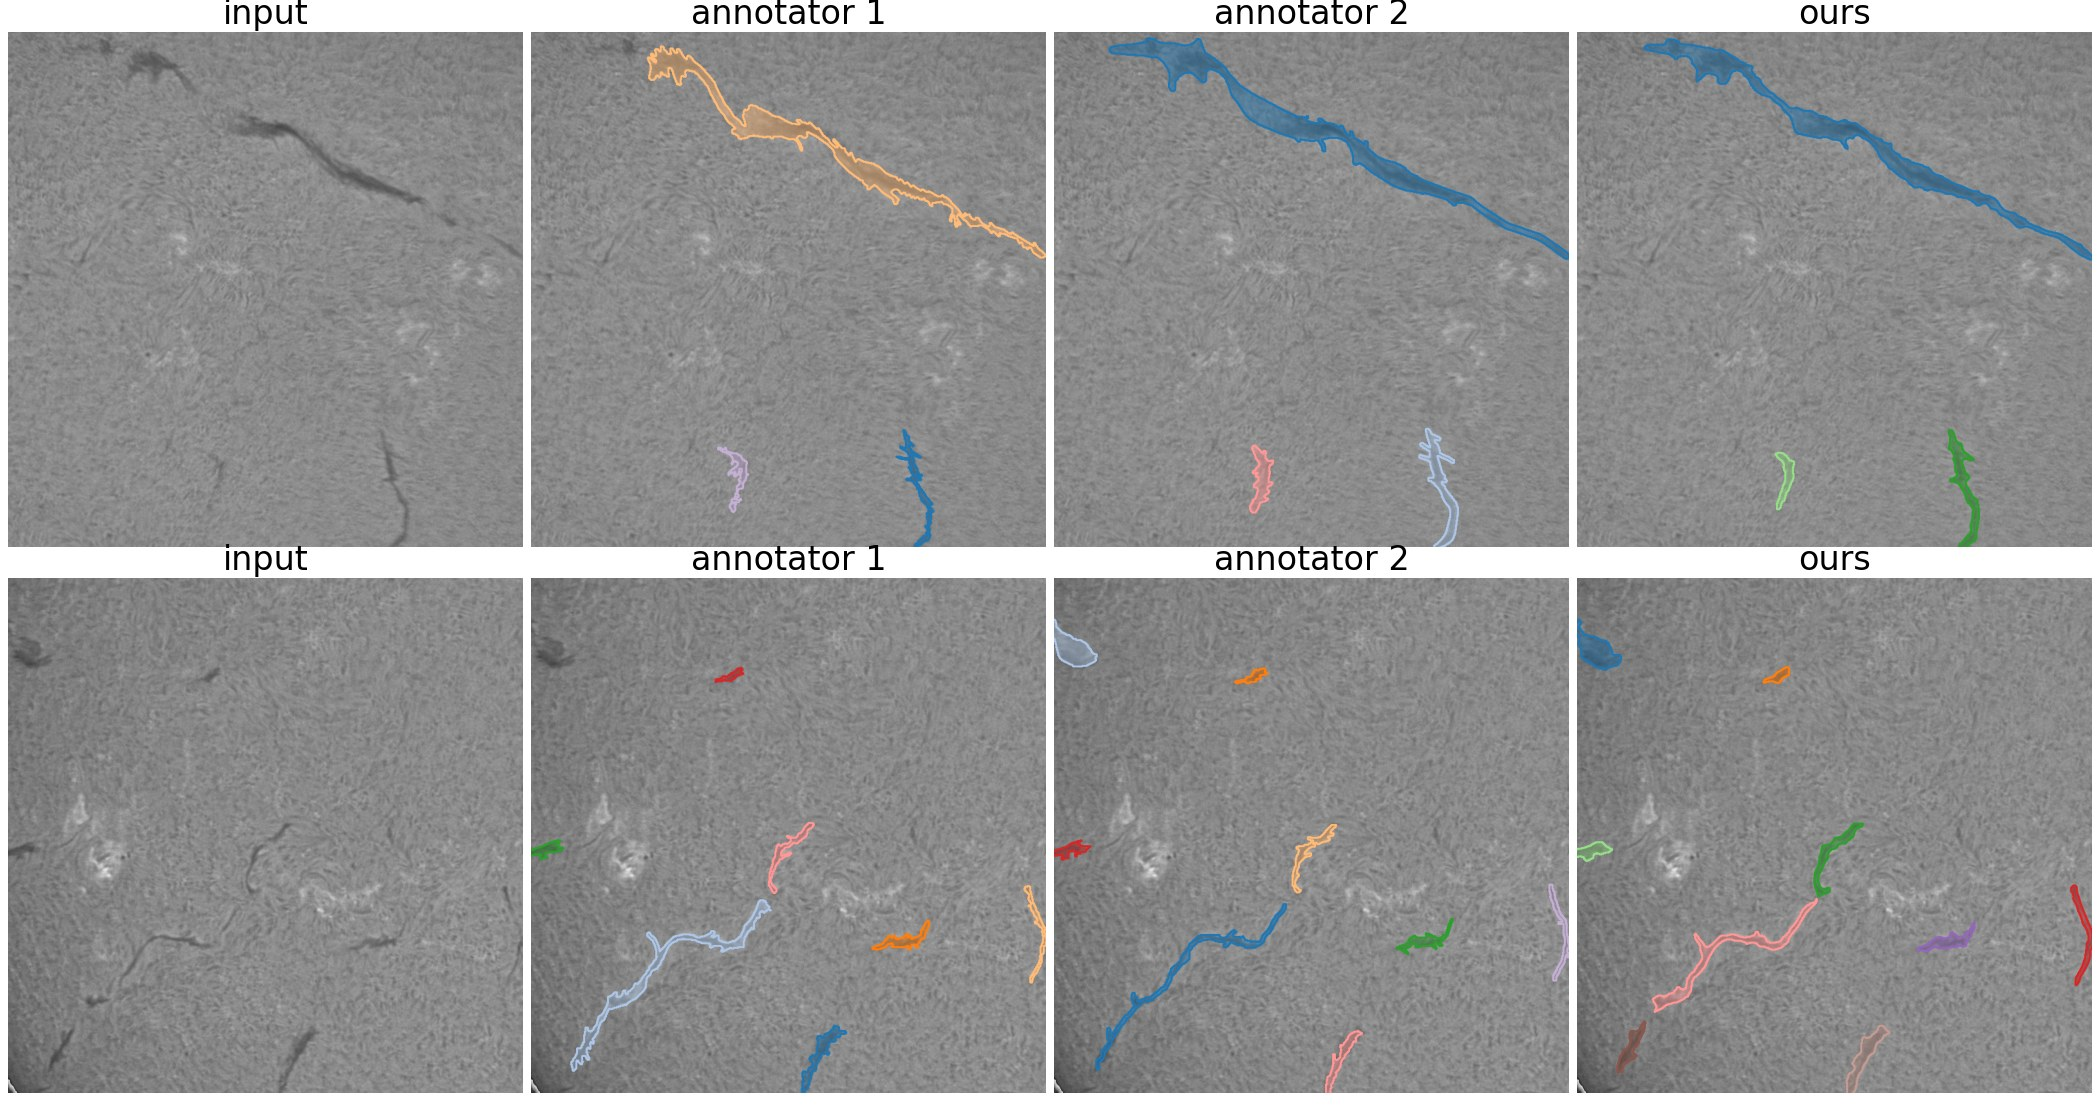
\includegraphics[width=\textwidth]{figures/qualitative.jpg}
\caption{Validation observations (800\,px crops of the 2048\,px frame), shown with two of their three annotators. Annotators disagree on extent and on which faint features count as filaments. Top: one long filament; our mask matches each of the three annotators (IoU 0.67--0.75) better than annotators 1 and 2 match each other (0.62). Bottom: most filaments are found; the tail of the long filament (bottom left) comes out as a separate instance, as annotator~3 (not shown) also drew it, while annotator~1 includes it in the long filament.}
\label{fig:qual}
\end{figure*}

\section{Experiments}
All runs in Table~\ref{tab:ablation} use the same split and scorer; epochs (15--60) and batch size differ between runs to fit memory and time, and post-processing is tuned per run on validation.

\begin{table}[t]
\caption{Validation PQ (144 observations, 248 views) and network time per image: forward pass, fp32, batch 1, median of 20 runs on an RTX 5070 Ti; multi-pass rows are the single pass times the number of passes. Semantic runs use components; instance runs use the D-FINE-seg instance head with greedy non-overlap. The submitted pipeline is in bold. $^*$Plus 80\,ms of CPU preprocessing.}
\label{tab:ablation}
\small
\begin{tabular}{@{}lrr@{}}
\toprule
Variant & PQ & ms \\
\midrule
\multicolumn{3}{@{}l}{\emph{Resolution and task (size S)}} \\
semantic, $1280^2$, argmax & 0.360 & 18 \\
instance, $1280^2$ & 0.397 & 19 \\
instance, $2048^2$ & 0.414 & 48 \\
semantic, $2048^2$, argmax & 0.417 & 50 \\
instance, trained on 1024 crops, 9 tiles & 0.421 & 123 \\
\midrule
\multicolumn{3}{@{}l}{\emph{Capacity (size M)}} \\
instance, $1024^2$ & 0.387 & 18 \\
semantic, $2048^2$ & 0.418 & 69 \\
\midrule
\multicolumn{3}{@{}l}{\emph{Semantic S, $2048^2$: post-processing}} \\
$p \geq 0.4$ & 0.419 & 50 \\
\textbf{$p \geq 0.4$ + component mean $p \geq 0.90$} & \textbf{0.429} & \textbf{50} \\
\quad + 8$\times$ flip/rotation TTA & 0.434 & 400 \\
\midrule
\multicolumn{3}{@{}l}{\emph{Semantic S, $2048^2$: labels and input (with the cut)}} \\
consensus labels (disagreement ignored) & 0.421 & 50 \\
union of views as label & 0.408 & 50 \\
limb-flattened + CLAHE input channels & 0.427 & 50$^*$ \\
\midrule
\multicolumn{3}{@{}l}{\emph{Other}} \\
instance + semantic fusion (best of 12) & 0.423 & 173 \\
instance $2048^2$ + 8$\times$ TTA & 0.428 & 382 \\
instance tiles + 8$\times$ TTA & 0.432 & 986 \\
\bottomrule
\end{tabular}
\end{table}

\textbf{Resolution dominates.} The native-resolution runs beat the best downscaled one (instance at $1280^2$) by +0.017 to +0.037 PQ; for the three runs we bootstrapped against it, the 95\% intervals lie above zero. Model size does not help at native resolution (M: 0.418 vs.\ S: 0.417) and cannot make up for resolution (M at 1024: 0.387). An instance model trained on native-resolution crops works only if inference uses the same scale (tiles: 0.421); on the full frame its confidences collapse (0.286).

\textbf{Task formulation is a tie.} At native resolution the instance and semantic formulations, and their fusion (instances group pixels, the semantic map draws boundaries), all lie within 0.009 PQ of each other, inside the noise. The semantic model is the simplest: no queries, no NMS, no mask overlap to resolve.

\textbf{Labels.} Training on per-view masks beats consensus targets (1 where all views agree, 0 where none mark filament, ignored otherwise): consensus raises SQ (0.682 vs.\ 0.675--0.677 for per-view training) but filaments drawn by only some annotators are never taught as positives, while they still count in the views that contain them. The union of views makes masks too wide (SQ 0.661). Limb-darkening flattening and CLAHE inputs add nothing: the network handles limb darkening from the raw frame.

\textbf{Test-time augmentation.} Averaging probabilities over the 8 flips and rotations adds +0.005 PQ (+0.0085 [+0.002, +0.015] without the cut) at 8$\times$ the network time; instance TTA reaches 0.432 at 20$\times$ the network time plus seconds of CPU post-processing per image. We submitted the single pass: its public score equals that of the TTA variant (both 0.38), and the speed matters for operational use.

\section{Results}

\begin{table}[t]
\caption{Rubric metrics on validation (pooled over 248 views), and the same metrics for annotators scored against each other on the same observations.}
\label{tab:rubric}
\small
\begin{tabular}{@{}lrr@{}}
\toprule
Metric & Ours & Annotators \\
\midrule
PQ & \textbf{0.429} & 0.334 \\
SQ (mean IoU of matches) & \textbf{0.675} & 0.631 \\
RQ (F1 of matches) & \textbf{0.635} & 0.530 \\
Mean image Dice & \textbf{0.668} & 0.633 \\
Mean Dice of matched filaments & \textbf{0.803} & 0.771 \\
One-to-many (\% of GT filaments) & 4.1 & 3.4 \\
Many-to-one (\% of predictions) & 3.4 & 3.4 \\
\bottomrule
\end{tabular}
\end{table}

\begin{figure*}[t]
\centering
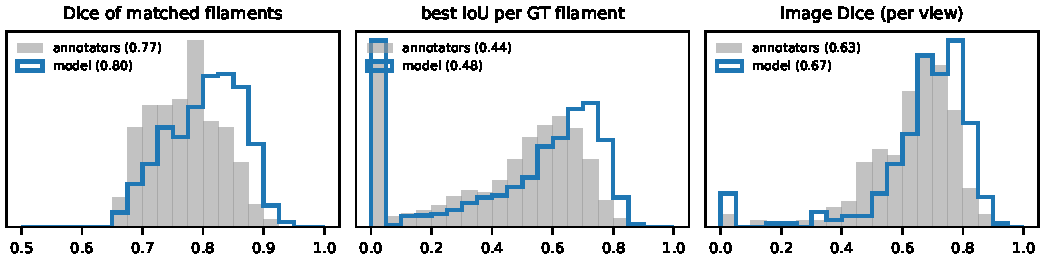
\includegraphics[width=\textwidth]{figures/distributions.pdf}
\caption{Validation distributions (means in the legends), ours (outline) vs.\ annotators scored against each other (grey). Left: Dice of matched filament pairs. Middle: best IoU of every ground-truth filament (0 = missed). Right: binary Dice per annotator view.}
\label{fig:dist}
\end{figure*}

Table~\ref{tab:rubric} and Fig.~\ref{fig:dist} show the rubric metrics. Our masks overlap the annotators' masks more closely than the annotators' overlap each other: matched Dice 0.80 vs.\ 0.77, and SQ 0.675 vs.\ 0.631. The model also finds more of each annotator's filaments (recall 0.61 vs.\ 0.53; RQ 0.635 vs.\ 0.530): it behaves like an average annotator, whereas each human draws a particular subset. Fragmentation and merging stay close to the annotators' level: 4.1\% of ground-truth filaments are touched by several predictions (annotators: 3.4\%), and 3.4\% of predictions touch several filaments (3.4\%). The spike at 0 in the middle panel is missed filaments, mostly small and faint ones. Recall (IoU $>0.5$) is 0.36 for filaments under 500\,px, 0.58 for 500--1000\,px and 0.70 above; annotators recover each other's filaments at 0.29, 0.45 and 0.61, so small filaments are where humans disagree most as well.

\textbf{Leaderboard.} The submission scores 0.38 on the public leaderboard, which uses about half of the 180 test images \cite{filament-segmentation-2026} and shows two decimals; the TTA and tiled-instance variants also score 0.38. This is 0.05 below validation, more than the spread across random halves of our validation set (standard deviation 0.012), so the public test images are harder or annotated differently than our split. The gap is consistent across all five variants we submitted (0.04--0.06), and their order is preserved: 0.397 on validation gives 0.35 public, 0.419 gives 0.36 and 0.421--0.434 give 0.38.

\textbf{Efficiency.} End to end, from a JPEG path to the final non-overlapping RLE masks, the pipeline takes 76\,ms per image (decode 11\,ms, network with softmax and transfer to the CPU 57\,ms, post-processing 9\,ms; RTX 5070 Ti, PyTorch, batch 1), with 1.5\,GB of peak allocated GPU memory (2.1\,GB reserved by PyTorch). The whole test set takes about 15\,s including model loading. Post-processing builds each component's RLE from its own pixels instead of encoding a full-frame mask per filament, which reduced it from 75\,ms to 9\,ms with byte-identical output. D-FINE-seg also exports the model to ONNX, TensorRT, OpenVINO and CoreML, which can lower the network time further, though we did not use this for the submission.

\section{Reproducibility}
The repository holds the code, training config, trained weights (32\,MB), submitted CSV, research scripts and a notebook that runs the whole pipeline. With the pinned \texttt{requirements.txt} (PyPI only, \texttt{dfine-seg==0.7.1}), \texttt{python -m filaments predict} regenerates the submitted file byte for byte. The model was trained with D-FINE-seg 0.6.1; the shipped config carries the same settings for 0.7.1. Only the competition's training annotations were used.

\section{Conclusion}
A single small real-time segmentation network at native resolution, with confidence-filtered connected components, agrees with the human annotators better than they agree with each other on PQ and Dice, at 76\,ms per image. Within our experiments the remaining PQ gains came only from ensembling-like averaging (TTA), at many times the compute, which suggests that the limit is now the consistency of the annotations rather than the model. For operational use on GONG frames we would keep the single pass.

\bibliographystyle{ACM-Reference-Format}
\bibliography{main}

\end{document}
